\documentclass[13pt]{article}
\usepackage[utf8]{inputenc}
\usepackage{amsmath}
\usepackage{comment}
\usepackage{physics}
\usepackage{mathrsfs}
\usepackage{graphics}
\usepackage{graphicx}
\usepackage{placeins}
\usepackage{caption}
\usepackage{subcaption}
\title{Varies aspect of Fano resonance}
\author{Shyamal Guchhait}
\date{October 2021}

\begin{document}

\maketitle

\begin{abstract}
    Enhancement of magneto-optical effects in hybrid magneto-plasmonic systems has attracted considerable recent attention because of their potential for building non-reciprocal nanophotonic devices. Quantitative understanding of the fundamental origin and contributing mechanisms for the enhancement is crucial for optimizing applications. Here, we unravel different physical origins of the giant enhancement of Faraday rotation and ellipticity in a hybrid magneto-plasmonic system, namely, waveguided magneto-plasmonic crystal for excitation with transverse electric (TE) and transverse magnetic (TM) polarized light. With TE polarization excitation, where the surface plasmons are not directly excited, the natural weak value amplification of Faraday effects appearing due to the spectral domain interference of Fano resonance is the dominant cause of the enhancement. For TM polarization excitation, on the other hand, waveguide-plasmon strong coupling and its universal manifestation of avoided crossing plays an important role, leading to maximum enhancement of the magneto-optical effects in the avoided crossing regime.
    \par
    The valley degree of freedom possessed by electronic excitations in transition metal dichalcogenides is providing new opportunities for information processing and optoelectronics. Valley contrasting polarization selection rules present unique opportunities for optical control in valleytronic devices. Critical to devices leveraging the valley degree of freedom is the ability to tailor optical valley polarizability and its degree of coherence. We are trying to measure valley coherence using spectral interference methods because interference is the primary method of measurement of coherence.
    \par 
    Monolayers of semiconducting transition metal dichalcogenides are two-dimensional direct-gap systems which host tightly bound excitons with an internal degree of freedom corresponding to the valley of the constituting carriers. Strong spin-orbit interaction and the resulting ordering of the spinsplit subbands in the valence and conduction bands makes the lowest-lying excitons in WX2 (X being S or Se) spin forbidden and optically dark. With polarization-resolved photoluminescence experiments performed on a WSe2 monolayer encapsulated in a hexagonal boron nitride, we show how the intrinsic exchange interaction in combination with the applied in-plane and/or out-of-plane magnetic fields enables one to probe and manipulate the valley degree of freedom of the dark excitons.
    
\end{abstract}
\section{Introduction}
\subsection{Magneto-plasmonic system}
\noindent
\par
	Hybridization of magneto-optic (MO) materials with plasmonic nanostructures enables magnetic-tuneable multifunctional nano-devices that is capable of providing precise control over its plasmonic and magnetic properties1,2. Moreover, such systems are also known to exhibit giant MO effects (Faraday, Kerr effect etc.)2,3,4,5,6,7,8. Note that the nonreciprocal nature of the MO effects is crucial for developing optical isolators3, modulators, and optical-magnetic data storage devices1,8 etc. Usually, the weak MO effects of the available materials are a major stumbling block towards their applications in nano scale devices. Significant efforts have therefore been delivered in the last few years to demonstrate enhancement of both the magneto-optical Kerr effect and the Faraday effect in magneto-plasmonic nanostructures2,4,7. Earlier approaches for increasing the MO activity of the systems were mostly based on the excitation of surface plasmons, where the near field enhancement associated with the surface plasmons leads to substantial enhancement of MO responses of samples9,10. In this regard, a recent study that has demonstrated giant enhancement of Faraday rotation in a waveguided magneto-plasmonic crystal (WMPC)3 system, has attracted a lot of attention. Subsequently, some other related studies have reported even larger enhancement of Faraday rotation in various magneto-plasmonic systems using similar approach4,6,11. In most of these studies, the enhancement of MO effects is attributed to either the surface plasmon-induced near field enhancement or to the coupling of the waveguide-plasmon-polariton2,4,6. For both the cases, the enhanced MO effect is related to the excitation of the surface plasmon resonance, which in case of the investigated planar structures can only be excited using transverse magnetic (TM) polarization of light. In contrast to this understanding, our recent investigation demonstrated a large enhancement of both the Faraday rotation and ellipticity in a Fano resonant WMPC system for incident TE polarized light where no surface plasmons were directly excited12. This observation indicated possibility of another important mechanism of the enhancement, namely, the natural weak value amplification (WVA) of Faraday rotation and ellipticity due to spectral domain interference of Fano resonance. Proper understanding of the different mechanisms of enhancement of the MO effects in hybrid magneto-plasmonic system and their dependence on the various physically accessible parameters of the system and of excitation light is of paramount importance for both fundamental and applied interests.

\par
	The concept of weak measurement and WVA was introduced by Aharonov, Albert, and Vaidman13,14,15,16,17. This special measurement process involves three steps, quantum state preparation (preselection), a weak interaction, and post-selection on a final quantum state that is nearly orthogonal to the initial state. The outcome of such measurement, the so-called weak value, may not only become exceedingly large and lie outside the eigenvalue spectrum of the observable but can also assume complex values13,14,15. The quantum mechanical concept of WVA can be understood within the realm of wave optics and thus most of the experiments on weak measurements are performed in classical optical setting17,18,19,20,21,22,23. The WVA concept can be interpreted as near destructive interference between the eigenstates of the measuring observable as a consequence of mutually near orthogonal pre and post selections of the system states13,14. Based on this simple interferometric philosophy of WVA, we had initially shown that a similar situation arises in the spectral domain interference of Fano resonance that leads to natural WVA of small Faraday rotation and ellipticity in WMPC12, which acts as the weak interaction in this scenario. An analytical model for natural WVA in Fano resonance demonstrating the amplification of small polarization anisotropic effects around the Fano destructive point was given in our previous publication. However, in the context of the WMPC, such a model12 was derived for a restricted case where the resonance frequencies for the TM and TE quasiguided modes are the same. Yet, it is important to investigate a more general scenario of natural WVA of Faraday effects in Fano interference, which is expected to provide a better understanding about the role of WVA in the enhancement of the MO properties in magneto-plasmonic crystals. Here, we have therefore addressed this issue by adopting differences in the resonance frequencies for the TE and the TM waveguide modes. This enabled us studying the dependence of the WVA of Faraday effects in Fano resonance (with TE polarization excitation) on the resonance frequencies of the TM and the TE modes and their varying extent of spectral overlap that can be tuned by changing the geometrical parameter of the plasmonic crystal system. In contrast to the TE polarization excitation, for the TM polarization excitation, the underlying physical mechanisms for the enhancement of the MO effects are expected to be rather complex and are more interesting due to simultaneous involvement and coupling of the waveguide mode and the plasmon mode in such hybrid system. As there appears to have different possible mechanisms of the enhancement of MO effects in magneto-plasmonic crystals2,3,4,10 including the one of natural WVA12, the question arises whether there is a common physical origin of the enhancement irrespective of the input polarization state or are there different mechanisms that contribute with varying strengths depending upon the excitation polarization and the geometrical parameters of the WMPC. The main purpose of this work is to address this important question and to shed light upon the competing roles of the different contributing mechanisms, namely, the natural WVA and the purity of Fano resonance12, near field enhancement effects due to the excitation of the surface plasmons2, resonance enhanced cross coupling between the TE and TM polarization3,4, the waveguide-plasmon strong coupling3,4, and the related phenomenon of avoided crossing and so forth on the giant enhancement of magneto-optical effects (Faraday rotation and ellipticity). The results of our study establish that while for TE polarization excitation, the natural WVA of Faraday effects due to Fano resonance is the dominant cause of the enhancement, for TM polarization excitation, the waveguide-plasmon strong coupling plays the leading role in the enhancement of the MO effects. This study also provides quantitative understanding on the observed giant enhancement of magneto-optical effects and provides potentially useful information on optimizing plasmonic crystal structure for its potential applications in nanoscale devices.
\subsection{Valley coherence in metal metal dichalcogenides system}
\noindent
\par 
	Nanoscale materials have attracted much attention in recent years for their potential to enable optoelectronic device architectures. Among these are monolayer transition metal dichalcogenides (TMDC)1,2. Monolayer TMDCs are direct bandgap semiconductors that support stable room-temperature excitons (binding energy of $0.3–0.5 eV$). The broken inversion symmetry and strong spin-orbit interaction give rise to pronounced optical selection rules at two energy-degenerate valleys3,4,5,6. The two valleys, $K$ and $K'$, can be activated by circularly polarized light with opposite handedness. As a result of the previous, the binary valley pseudospin index has been identified as potential information bearing degree-of-freedom (DOF) giving birth to the field of valleytronics7,8.
	In analogy to spintronics, valleytronics relies on the ability to store, manipulate and readout information from the valley pseudospin. To date, the optical pumping of valley polarization3,4,5,6 and the optical generation, and manipulation of valley coherence have been observed at cryogenic temperatures9,10,11,12,13. However, the major obstacle to coherently controlling the valley DOF at room temperature is the intervalley dephasing processes mediated by phonons, the electron-hole interaction or the Maialle-Silva-Sham mechanism (MSS mechanism)14.

	Recent work has demonstrated the potential to realize cavity polaritons based on TMDCs15,16,17,18. It has been discovered that TMDC polaritons inherit the valley DOF and exhibit enhanced valley polarization at elevated temperature19,20,21,22. In this work we leverage polaritons based on the monolayer tungsten diselenide (WSe2) to circumvent intervalley dephasing and preserve finite valley coherence at room temperature. The polariton valley coherence is studied by steady-state angle-resolved Photoluminescence (PL) measurements (See Supplementary Note 1) and explained by a valley-resolved Jaynes–Cummings model23,24 (See Supplementary Note 2). Our results provide a path to realizing room-temperature valleytronic devices.
\par 
\begin{comment}
Monolayers (MLs) of semiconducting transition metal dichalcogenides (TMDs), such as MX2 with M ¼ Mo or W, and X ¼ S, Se, or Te, are two-dimensional direct-gap semiconductors [1] which attract a lot of interest due to their unique physical properties and potential applications in optoelectronics, photonics, and the development of valleytronics [2–7]. The direct band gap in S-TMD MLs is located at the two inequivalent K points (valleys) of the
first Brillouin zone, related by time reversal symmetry. In MLs, the optically bright excitons [8–11] from K valley can efficiently couple to light with right or left circular polarization[12,13], respectively. A unique feature of S-TMD monolayers is the so-called spin-valley locking [13]: strong spin-orbit interaction lifts the degeneracy between the two spin projections s ¼ ↑; ↓ in each valley, leaving only the Kramers degeneracy between the opposite valleys, Kþ; s ↔ K−;−s. While the valence band (VB) spin-orbit splitting Δv is very large (several hundred meV [13]), its conduction band (CB) counterpart Δc is by an order of magnitude smaller [14–18], thus allowing some degree of manipulation by an in-plane magnetic field. In tungsten-based S-TMDs, Δc has the same sign as Δv, leading to the spin subband ordering shown in Fig. 1(a). In each valley, the optically bright exciton has a higher energy than the dark exciton which is composed of the conduction and valence electronic states with opposite spin projections. This results in a strong temperature (a) (b) FIG. 1. (a) Spin and valley structure of WSe2. Black curves show the spin-split bands in th eK valleys at zero magnetic field, the spin projections are indicated by black arrows. Grey (red) ellipses represent spin-forbidden (spin-allowed) excitonic transitions in each valley. Dashed green curves show Zeeman-shifted bands in a perpendicular magnetic field. Thick green arrows represent the exchange interaction which mixes the two valleys, and the Zeeman coupling in an in-plane magnetic field which mixes different spin subbands in the same valley. (b) A schematic representation of radiation patterns of dark and bright excitons in a ML at zero magnetic field. The grey (red) arrows indicate the propagation direction of the light, emitted by dark (bright) excitons. The blue dashed lines define the region of light collected by the lens. The black and red double-headed arrows depict the directions of out-of-plane (d⊥) and in-plane (dk) dipoles dependence of the photoluminescence (PL) efficiency, as the bright states become more populated at higher temperatures [19–21].
\end{comment}

\section{Theory \& Methods}
\subsection{ Theoretical framework of natural WVA of Fara-day effects in a Fano resonant WMPC}
\noindent
\par
	Our natural weak value amplification (WVA) formalism is founded on a simple but intuitive model of optical Fano resonance that uses coherent interference of a narrow resonance mode described by a complex Lorentzian with a frequency-independent continuum (or broad) mode1,2. It has been  observed earlier that similar simple model can capture the near field mode coupling and the Fano interference  effect  in  various  optical  systems including  the  plasmonic  crystals3–8.  The  resultant Fano scattered electric field is given by
\begin{equation}
	\centering
	E_s(\omega) \approx \left[ \frac{q - i}{\varepsilon + i} +B \right] = \left[ \sqrt{\frac{q^2 +1}{\varepsilon^2 +1}} e^{i\Psi(\omega)} +B\right]
	\label{eqs:WVA Electric field}
\end{equation}

	The total phase difference between two interfering modes $\Psi(\omega)$ is

\begin{equation}
	\centering
	\Psi(\omega) = \arctan{\frac{q - \varepsilon}{1 + q\varepsilon}}
	\label{eqs:WVA Electric field phase}
\end{equation}

	The resulting expression for the transmitted intensity of electric field described in Eq. \ref{eqs:WVA Electric field} can be  obtained as 

\begin{equation}
	\centering
	I_S(\omega) = \abs{E_S(\omega)}^2 = B^2 \times \left[ \frac{(q^{eff} + 1)^2}{\varepsilon^2 + 1} \right] + \frac{(B - 1)^2}{\varepsilon^2 + 1}
	\label{eqs:WVA Eletric intensity}
\end{equation}

The parameter $B$ is the relative amplitude of the continuum with respect to the field of the narrow resonance and determines the contrast of the spectral domain interference. For the ideal situation of $B = 1$ the  perfect  destructive  interference  occurs  at  the  Fano  frequency $\omega_F = \left( \omega_0 - \frac{q\gamma}{2} \right)$ corresponding to $(\varepsilon = -q, \Psi(\omega_F) = \pi)$
Here  we  are  proposing  a  generalized  model  of  Fano  interference  in  the  WMPC  by  considering different resonant frequencies for TE and TM waveguide modes. The resultant polarized field can be expressed as

\begin{multline}
	E_s(\omega) \approx \left[ \frac{q - i }{\varepsilon(\omega)^{TE} + i} (\cos(\alpha)\cos(\chi) - i\sin(\alpha)\sin(\chi)) \hat{y} + \right. \\
	\left. \frac{q - i }{\varepsilon(\omega)^{TM} + i} (\sin(\alpha)\cos(\chi) - i\cos(\alpha)\sin(\chi)) \hat{x} + B \hat{y} \right]
	\label{eqs:WVA Electric field Fano}
\end{multline}

	Here, $\varepsilon(\omega)^{TE} = \frac{\omega - \omega_{0}^{TE}}{\frac{\gamma}{2}}$, $\varepsilon(\omega)^{TM} = \frac{\omega - \omega_{0}^{TM}}{\frac{\gamma}{2}}$ where $\omega_{0}^{TE}$ and $\omega_{0}^{TM}$ are the resonance frequencies of the TE and the TM waveguide modes respectively and $\gamma$ is the width of the resonance, which is assumed to be of similar magnitude. The $q$ parameter is related to the coupling of the modes and determines the characteristic asymmetry of Fano spectral line shape. In this model, the spectral domain interference of the modes can be understood through the phase difference between them, which is very important for our weak value analysis

\begin{subequations}
	\centering
	\begin{equation}
		\centering
		\Psi(\omega)^{TE} = \arctan \left[ \frac{q + \epsilon^{TE}}{1 -q\epsilon^{TE}} \right]
	\end{equation}
	\begin{equation}
		\centering
		\Psi(\omega)^{TM} = \arctan \left[ \frac{q + \epsilon^{TM}}{1 -q\epsilon^{TM}} \right]
	\end{equation}
	\label{eqs:WVA total phase}
\end{subequations}
	$\Psi(\omega)^{TE/TM}$ is  the  total  phase  difference  between  the  waveguide  mode  (TE/TM)  and  the  broad continuum. For an ideal continuum $(B = 1)$ the exact destructive interference occurs at the Fano frequency $\omega_F = \omega_0^{TE} - \frac{q\gamma}{2}$ corresponding to $\varepsilon^{TE} = -q$. Note that $\omega_F$ is the frequency of exact destructive  interference,  where  the  phase  difference  between  the  TE  quasiguided  mode  and incoming broad continuum becomes $\Psi(\omega_F)^{TE} = \pi$ and the ratio of the amplitudes between them is  unity $a(\omega_F) = 1$. At  close  vicinity  of $\omega_F$, near  destructive  spectral  interference  takes  place between  the  two  modes  with  simultaneous  small  amplitude  offset $(\epsilon_a(\omega))$ and  phase  offset $(\epsilon_p(\omega))$. It is this near destructive spectral interference between the two modes that mimics the near  orthogonal  pre  and  post-selections  of  states  (small  overlap  of  states $\epsilon_(a/p)$ )  in  conventional optical  WVA.  It’s  important  to  note  that,  in  the  general  case,  the  amplitude  and  phase  offset parameters  for  TE $(\epsilon_{a/p})$  and  TM $(\epsilon^{'}_{a/p})$ interfering  modes  will  differ  owing  to  their  different resonance frequencies, which can be expressed as (expression is given in Eq. 2 and Eq. 3 of the manuscript).
\begin{subequations}
	\centering
	\begin{equation}
		\epsilon_a(\omega) \approx \frac{\left( 1 - \sqrt{\frac{\varepsilon^2 + 1}{q^2 + 1}} \right)}{\left( 1 + \sqrt{\frac{\varepsilon^2 + 1}{q^2 + 1}} \right)}        
	\end{equation}
	\begin{equation}
		\epsilon_p(\omega) = \pi - \Psi(\omega) = \pi - \arctan{\left(\frac{q - \varepsilon}{1 + q\varepsilon}\right)}
	\end{equation}
	\label{}
\end{subequations}

	However, in the general case, the amplitude and phase offset parameters for TE $( \epsilon_{a/p} )$ and TM $( \epsilon^{'}_{a/p} )$ interfering modes will differ owing to their different resonance frequencies, which can be expressed as 

\begin{subequations}
	\centering
	\begin{equation}
		\epsilon_a(\omega) \approx \frac{\left( 1 - \sqrt{\frac{\varepsilon^2 + 1}{q^2 + 1}} \right)}{\left( 1 + \sqrt{\frac{\varepsilon^2 + 1}{q^2 + 1}} \right)}        
	\end{equation}
	\begin{equation}
		\epsilon_p(\omega) = \pi - \Psi(\omega)^{TE} = \pi - \arctan{\left(\frac{q - \varepsilon}{1 + q\varepsilon}\right)}
	\end{equation}
	\begin{equation}
		\varepsilon(\omega) = \frac{\omega - \omega_0^{TE}}{\frac{\gamma}{2}}
	\end{equation}
	\label{}
\end{subequations}

\begin{subequations}
	\centering
	\begin{equation}
		\epsilon^{'}_a(\omega) \approx \frac{\left( 1 - \sqrt{\frac{\varepsilon^2 + 1}{q^2 + 1}} \right)}{\left( 1 + \sqrt{\frac{\varepsilon^2 + 1}{q^2 + 1}} \right)}        
	\end{equation}
	\begin{equation}
		\epsilon^{'}_p(\omega) = \pi - \Psi(\omega)^{TM} = \pi - \arctan{\left(\frac{q - \varepsilon}{1 + q\varepsilon}\right)}
	\end{equation}
	\begin{equation}
		\varepsilon(\omega) = \frac{\omega - \omega_0^{TM}}{\frac{\gamma}{2}}
	\end{equation}
	\label{}
\end{subequations}

Now  the  WVA  of  polarization  rotation  $\alpha$ and  ellipticity $\chi$ will  depend  on  both  the  offsets $\epsilon_(a/p)^{TE}, \epsilon_(a/p)^{TM}$ Using the framework of WVA considering two different amplitude and phase  offsets,  the  resultant  Fano  scattered  electric  field  described  in  Eq.  \ref{eqs:WVA Electric field} can  be  written  in  terms  of  simultaneously varying  offset parameters $(\epsilon_(a/p), \epsilon^{'}_(a/p))$. In this  complex  WVA scenario it can  be written as

\begin{multline}
	E_s(\omega) = \left[ (1 + \epsilon_a) e^{i\epsilon_p} \{ (\cos(\alpha)\cos(\chi) - i\sin(\alpha)\sin(\chi)) \hat{y} + \right. \\
	\left. (1 + \epsilon^{'}_a) e^{i\epsilon^{'}_p} (\sin(\alpha)\cos(\chi) - i\cos(\alpha)\sin(\chi)) \hat{x} \} + \right. \\
	\left. (1 - \epsilon_a) e^{-i\epsilon_p} \hat{y} \right]
	\label{eqs:WVA Electric field offset}
\end{multline}
	Here $\epsilon_a$ and $\epsilon_p$ are the amplitude and phase offsets of the TE waveguide mode and the  $\epsilon^{'}_a$ and $\epsilon^{'}_p$ corresponds to the offsets of the TM waveguide mode which can be calculated using Eq. 3 of the manuscript.  The simultaneous real and imaginary WVAs of polarization rotation $\alpha$ and ellipticity $\chi$ are  manifested  in  the $\epsilon_{a/p}$ and $\epsilon^{'}_{a/p}$ dependent  large  observed  polarization  vector  orientation angle $\psi$ (determined from the $U$ and $Q$ tokes parameters10), and the circular (elliptical) polarization descriptor $4^{th}$ Stokes vector element $\frac{V}{I}$. As the TE and TM waveguide modes moves away from each other one cannot approach a very small value of amplitude and phase offsets for both  the  waveguide  modes $(\epsilon_{a/p}^{TE} \rightarrow 0, \epsilon_{a/p}^{TM} \rightarrow 0)$ simultaneously,  which  is  very  much desirable for optimal weak value amplification. Consequently, the maximum achievable amplification  of  polarization  rotation $\alpha$ and  ellipticity $\chi$ gets  limited.  In  contrast,  for  the  ideal WVA scenario $(\omega_0^{TE} = \omega_0^{TM} = \omega_0)$ the conditions of getting very small offsets are met for both the waveguide modes $(\epsilon_{a/p}^{TE} \rightarrow 0, \epsilon_{a/p}^{TM} \rightarrow 0)$ around the Fano dip $\omega_F$ leading to the maximum  achievable  amplification.  Some  results  are  presented  below  using  Eq.  S4 and  Eq.  S6 demonstrating  the  behaviour  of  natural  WVA  with  varying  overlap  between  the  TE  and  TM waveguide modes.

\subsection{Valley coherence theoretical model}
\noindent
\par 
	Interference is the basic measurement of the coherence of light. Photo lumination (PL) is a traditional method of valley coherence. Fano resonance is a type of resonant scattering phenomenon that gives rise to an asymmetric line shape. Spatial interference between two resonant scattering modes produces an asymmetric line shape. In our model, we used metal dichalcogenides on top of the glass surface. We used metal dichalcogenides like MoSe2, WSe2, etc. this type of material has valley coherence. The broad light spectrum incident on this material due to the valley gets a very narrow resonance. This narrow resonance interference with the refraction light from the glass surface forms an asymmetric line shape. The Fano resonance equation for this system is 
\begin{equation}
	\centering
	I_0 = \frac{(\eta \sqrt{x} q +\epsilon)}{\epsilon^2 + 1} + 
	\frac{q^2 (1 - \eta^2 x) + 2 (1 - \eta \sqrt{x})}{\epsilon^2 + 1}
	\label{eqs:valley coherence Fano equation}
\end{equation}
	Here $q$ \& $\epsilon$  are the Fano asymmetric parameter and reduce energy respectively. $\eta$ \& $x$ are the coherence of the incident beam and degree of polarization (valley coherence) respectively. 
\par 
Condition for minimum intensity $(I_{min})$ is $\epsilon = -q$
\begin{equation}
	\centering
	I_{min} = 2(1 - \sqrt{x} \eta)
\end{equation}
	Condition of the maximum intensity $I_{max}$ is $\epsilon = \frac{1}{q}$
\begin{equation}
	\centering
	I_{max} = 1 + q^2
\end{equation}
Visibility $(\mathscr{V})$ is 
\begin{equation}
	\centering
	\mathscr{V} = \frac{(q^2 + 1) - 2 (1 - \sqrt{x} \eta)}{(q^2 + 1) + 2 (1 -\sqrt{x} \eta)}
\end{equation}
	Here $x = \eta_{valley}$ and the $\sqrt{x} \eta$ is $\eta_{net}$
\begin{equation}
	\centering
	\eta_{net} = \sqrt{x} \eta
	\label{eqs:eta_net}
\end{equation}
\begin{equation}
	\centering
	\mathscr{V} = \frac{(q^2 + 1) -2 (1 -\eta_{net})}{(q^2 + 1) +2 (1 - \eta_{net})}
\end{equation}

\section{Result \& Discussion}
\noindent
\par 
\subsection{Enhancement of MO effects in WMPCs for TE polarization excitation as a manifestation of interferometric natural WVA in Fano resonance.}
\noindent
\par
	The WMPC system comprises of a periodic array of noble metal nanostructures on top of a dielectric waveguiding layer, which is made of MO materials that exhibit Faraday rotation and ellipticity. The coupling of the spectrally broad surface plasmon mode in the metallic nanostructures or the photon continuum (depending upon the excitation polarization of light) with the narrow quasiguided photonic modes in the waveguiding layer leads to Fano resonance. We used finite element method (FEM)26 for simulating the polarization resolved transmittance spectra from such system (see Methods). A schematic illustration of the FEM simulation of transmission and MO spectral responses of the WMPC is presented in Fig. \ref{fig:figure1} 
\begin{figure}[hbt!]
	\centering
	\begin{subfigure}[]{.49 \linewidth}
		\centering
		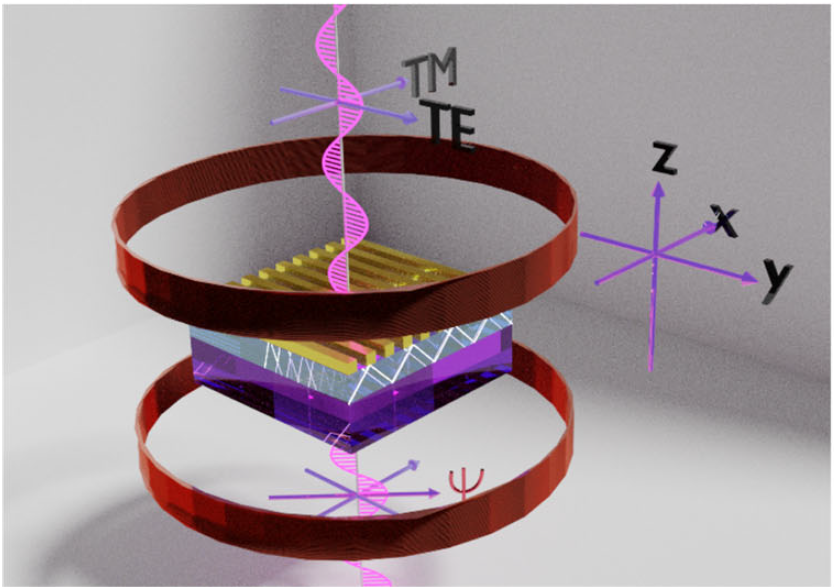
\includegraphics[width=\linewidth, height=140px]{Figures/figure1a.png}
		\caption{}
		\label{}
	\end{subfigure}
	\hfill
	\begin{subfigure}[]{.49 \linewidth}
		\centering
		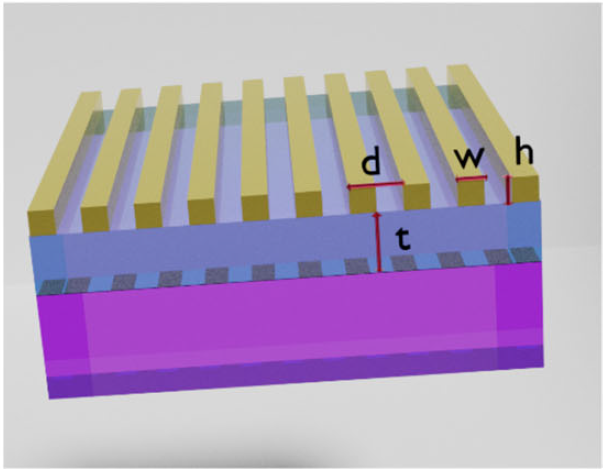
\includegraphics[width=\linewidth, height=140px]{Figures/figure1b.png}
		\caption{}
		\label{}
	\end{subfigure}
	\caption{\textbf{The waveguide magneto-plasmonic crystal (WMPC).} \textbf{a} A schematic illustration of the finite element method (FEM) simulation of Faraday rotation $\psi$ in the transmission spectra of the WMPC system. The direction of the transverse magnetic TM $(x)$ and transverse electric TE $(y)$ polarized light electric fields are perpendicular and parallel (respectively) to the axis of the Au gratings in the WMPC. \textbf{b} The WMPC system comprises of gold $(Au)$ gratings on top of a thin yttrium-bismuth iron garnet $(Y-BIG)$ film and the substrate is taken to be quartz. The Y-BIG film serves as the waveguiding layer and additionally exhibit Faraday effect in the presence of an external magnetic field. The thickness of the Y-BIG film $(t)$ and the periodicity $(d)$, width $(w)$, and height $(h)$ of the $Au$ gratings are marked.}
	\label{fig:figure1}
\end{figure}
\FloatBarrier
	The WMPC system investigated in this study consists of gold (Au) grating on top of a thin yttrium-bismuth iron garnet (Y-BIG) film and the substrate is taken to be quartz. The MO active Y-BIG film serves as the waveguiding layer and also exhibits Faraday effect in the presence of an external magnetic field (see Methods). The simulated transmittance spectra $(E = \hbar \omega 0.83 to 2.067 eV)$ and Faraday rotation and ellipticity for varying geometrical parameters of the WMPC with TE polarization excitation are summarized in Fig. 2. The transmission spectra (Fig. 2a, e, i), the spectral variation of the observed Faraday rotation $\psi$ (Fig. 2b, f, j) and the observed net ellipticity $\xi$ (Fig. 2c, g, k) of the WMPC are shown for varying periodicity d (Fig. 2a, b, c), width $w$ (Fig. 2e, f, g) and height $h$ (Fig. 2i, j, k) of the Au grating. Several observations can be made. Prominent signatures of Fano resonance with asymmetric spectral line shape are observed in all the transmission spectra with TE polarization excitation (Fig. 2a, e, i). Here, the surface plasmons are not directly excited and hence the Fano resonance27–29 arises due to the interference between the spectrally narrow quasiguided resonance mode with an ideal photon continuum. Importantly, giant enhancement of Faraday rotation (Fig. 2b, f, j) and ellipticity (Fig. 2c, g, k) are observed around the Fano spectral dip $(E = \hbar \omega_F )$ for all the geometrical parameters of the WMPC. In agreement with previous reports30, the Fano spectral dip is observed to gradually move towards shorter frequency (or energy $E = \hbar \omega$ ) with increasing periodicity $(d)$ of the grating (Fig. 2a). The magnitudes of the enhanced Faraday rotation $\psi$ (Fig. 2b) and ellipticity $xi$ (Fig. 2c) exhibit an interesting trend with varying $d-$ these increase to a maximum value for a certain value of periodicity and then follow a gradual decrease. The maximum magnitudes of the enhanced Faraday rotation $(\psi \sin 1:551)$ and ellipticity $(\xi \sin 1.559 )$ of the WMPC are obtained for a value of $d = 550 nm$ (Fig. 2b), as compared to the corresponding average bare film rotation and ellipticity of $0.28$ and $0.1$; respectively. Neither the value of the width $w$ nor the height $h$ of the Au grating has any significant influence on the quasiguided modes and hence the resulting Fano spectral line shape of the WMPC is not sensitive to variations of the w and the hparameters of the grating (Fig. 2e, i). Accordingly, the magnitude and spectral variation of both the Faraday rotation (Fig. 2j) and ellipticity (Fig. 2k) do not exhibit appreciable variation with the change in the height h of the grating. Similarly, with varying width $w$ of the grating, the Faraday rotation $\psi$ (Fig. 2f) and ellipticity $\xi$ (Fig. 2g) exhibit only weak variations (Faraday effects seem to be marginally stronger for w = 120 nm as compared to others). The spectral variation of the transmitted TM polarization intensities with TE polarization excitation are also plotted for each of the varying geometrical parameters of the WMPC (Fig. 2d, h, l). In general, the TM polarized intensities are considerably weak and approach their respective minima near the Fano spectral dip where maximum magnitudes of Faraday rotation and ellipticity are observed. This rule out the possibility of the role of the resonance enhanced cross-coupling of the TE and the TM quasiguided modes in the enhancement of the Faraday effect. The observed enhancement of the Faraday rotation and ellipticity around the Fano spectral dip corresponding to near destructive spectral domain interference between the quasiguided mode and the photon continuum is thus indicative of the prominent role of the natural WVA of Fano resonance for TE polarization excitation. This aspect is therefore investigated in further details by studying the dependence of the Faraday effect enhancement on the periodicity of the grating and through its natural weak value interpretation. As we proceed further, we note that we have also provided the near field distribution of both the TE and the TM polarizations around the Fano spectral dip (Supplementary Fig. 3), which confirms the dominance of the TE polarized field and the waveguiding nature of both the TE and the TM polarized fields around the Fano dip (see Supplementary Note 3 for details). 
	
\begin{figure}[hbt]
	\centering
	\begin{subfigure}[]{.49\linewidth}
		\centering
		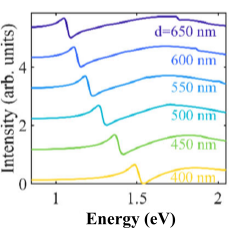
\includegraphics[width=\linewidth]{Figures/figure2a.png}
		\caption{}
		\label{}
	\end{subfigure}
	\hfill
	\begin{subfigure}[]{.49\linewidth}
		\centering
		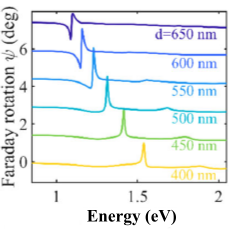
\includegraphics[width=\linewidth]{Figures/figure2b.png}
		\caption{}
		\label{}
	\end{subfigure}

	\begin{subfigure}[]{.49\linewidth}
		\centering
		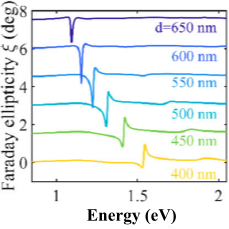
\includegraphics[width=\linewidth]{Figures/figure2c.png}
		\caption{}
		\label{}
	\end{subfigure}
	\hfill
	\begin{subfigure}[]{.49\linewidth}
		\centering
		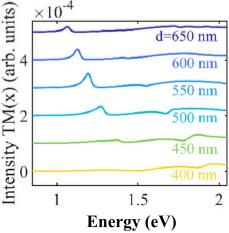
\includegraphics[width=\linewidth]{Figures/figure2d.png}
		\caption{}
		\label{}
	\end{subfigure}
	\caption{}
	\label{}
\end{figure}
\end{document}
